\documentclass{article}
\textheight 20.5truecm \textwidth 14.5truecm
\setlength{\oddsidemargin}{0.35in}\setlength{\evensidemargin}{0.35in}

\usepackage[utf8]{inputenc}
\usepackage[russian]{babel}
\usepackage{graphicx}
\usepackage{amsmath}
\usepackage{breqn}
\usepackage{wrapfig}
\usepackage{float}
\usepackage{multirow}
\usepackage{caption}
\usepackage{subcaption}

\graphicspath{ {./data/images} }
\author{Александр Романов Б01-110}
\date{}
\title{10.1 Электронный парамагнитный резонанс}

\begin{document}
\maketitle
\section{Введение}
\subsection{Краткое описание}
Исследуеься электронные парамагнитный резонанс в молекуле ДФПГ, определяется \(g\)-фактор электрона,
измеряется ширина линии ЭПР.

\subsection{Экспериметнальная установка}
\begin{figure}[H]
	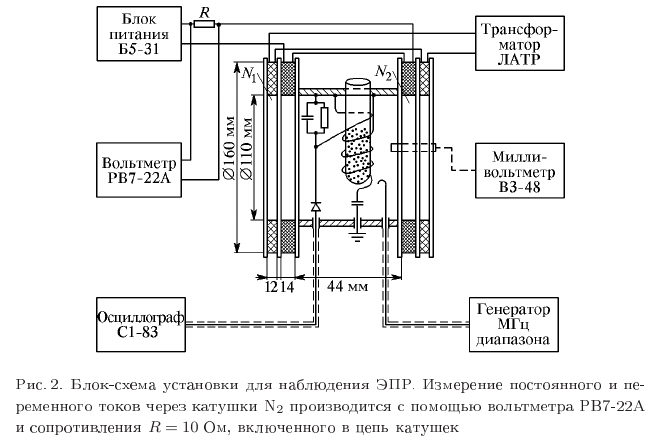
\includegraphics[width=\textwidth]{scheme.png}
\end{figure}
\section{Работа}
\subsection{Получение сигнала ЭПР на свободном радикале ДФПГ и измерение \(g\)-фактора электрона}
Включим и настроим генератор и осциллограф и получим на экране картину модулированных колебаний. 
Включим питание основных катушек от источника постоянного тока и питание модулирующих катушек 
-- через автотрансформатор -- от сети переменного тока 220В. 
Установим на модулирующих катушках напряжение около 50В. Плавно меняя реостатом величину тока,
проходящего через основные катушки, найдём сигнал ЭПР. Отрегулируем величину тока так, чтобы 
расстояние между пиками резонанса на экране осциллографа было одинаковым:

\begin{figure}[H]
	\centering
	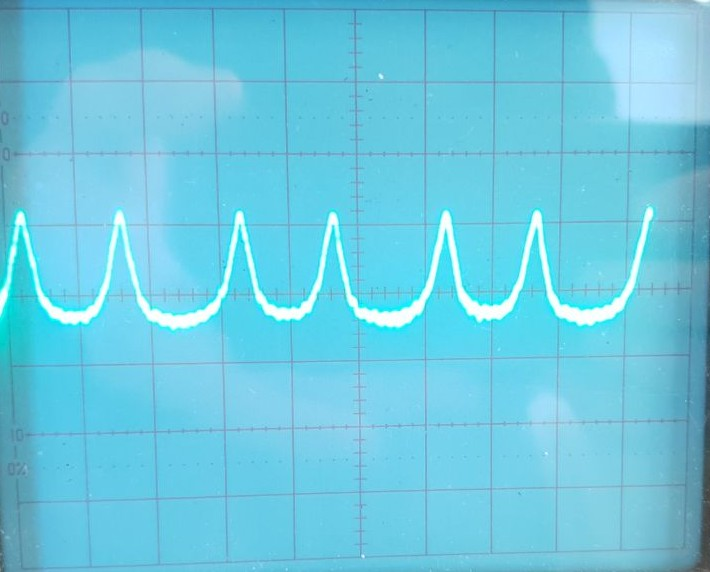
\includegraphics[width=0.7\textwidth]{Peaks.jpeg}
\end{figure}

Включим вилку питания пробной катушки в клеммы автотрансформатора. Измерим величину переменного поля. 
Для этого введём пробную катушку внутрь основных катушек поблизости от образца. И запишем показания
вольтметра: \(V = 140\; mV\). Зная число витков (\(n = 45\)) и площадь сечения 
(\(S = \frac{\pi D^2}{4} = 176\cdot 10^{-6}\; m^2 \)) пробной катушки определим напряжённость поля:

\[B_0 = \frac{v}{nS\omega_{\simeq}} = \frac{V}{ns \cdot 2\pi\nu_{net}} = 0.0047\;\text{эрстед}\]

Теперь вычислим \(g\)-фактор электрона (Частота резонанса: \(\omega_0 = 160.5 \pm 0.1 MHz\)):
\[ g = \frac{\hbar\omega_0}{\mu_{\text{Б}}B_0} = 2.03 \pm 0.04 \]

\subsection{Определение ширины линии ЭПР}
Получив сигнал ЭПР на ДФПГ в прошлом пункте, переключим осциллограф с временной развёртки на развёртку
от модуляционных катушек. Длина развёртки соответсвует удвоенной амплитуде модулирующегося поля:

\begin{figure}[H]
	\centering
	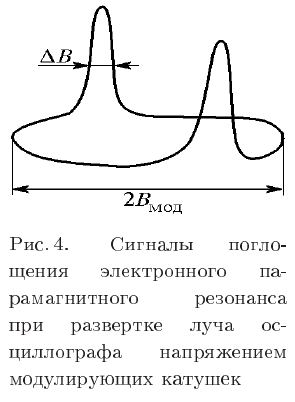
\includegraphics[width=0.3\textwidth]{2B.png}
\end{figure}

\begin{figure}[H]
	\centering
	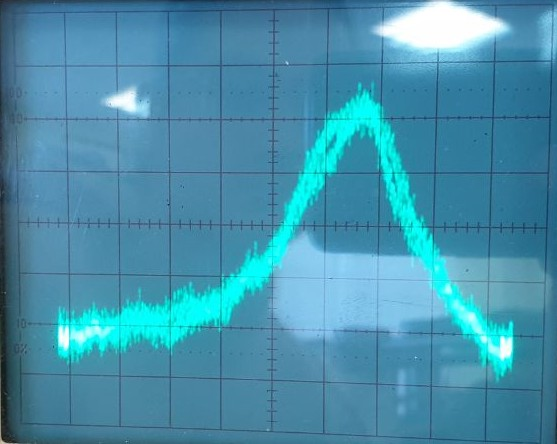
\includegraphics[width=0.7\textwidth]{Osc.jpeg}
\end{figure}

Измерим ширину по экрану осциллографа. \(\Delta l = 2.6 - 0.2 = 2.4 \pm 0,1\)
При этом амплитуда поля измеряется так же, как и в первом пункте: 
\[B_0 = 9.5\; \text{мТл}\]
Получим:
\[ \frac{\Delta B}{1\;\text{мТл}} = /frac{2.4}{9.6} \]
Отсюда:
\[\Delta B = 0.25\;\text{мТл}\]
Что сильно меншье поля Земли. Приемлемо.
\section{Выводы}
В ходе выполнения работы:
\begin{enumerate}
	\item Было экспериментально получено значение \(g\)-фактора электрона (\(g = 2.03 \pm 0.04\)). Полученное значение совпадает с теоретическим (\(g = 2\))
\end{enumerate}
\end{document}
